% Splitting of Hydrogen in different strong magnetic fields
% Author: Stephan Fuchs, Uni Bonn
\documentclass{standalone}
\usepackage{tikz}
%%%<
\usepackage{verbatim}
%%%>
\begin{comment}
:Title: Splitting of Hydrogen in different strong magnetic fields
:Tags: decorations;physics;chemistry
:Author: Stephan Fuchs
:Slug: hydrogen-splitting
This picture shows the splitting of Hydrogen in different
strong magnetic fields.

The "standalone" class has been used to fit the paper canvas
to the big picture.
\end{comment}
\usetikzlibrary{decorations.pathmorphing}
\usetikzlibrary{arrows}
\usepackage{nicefrac}
\begin{document}
  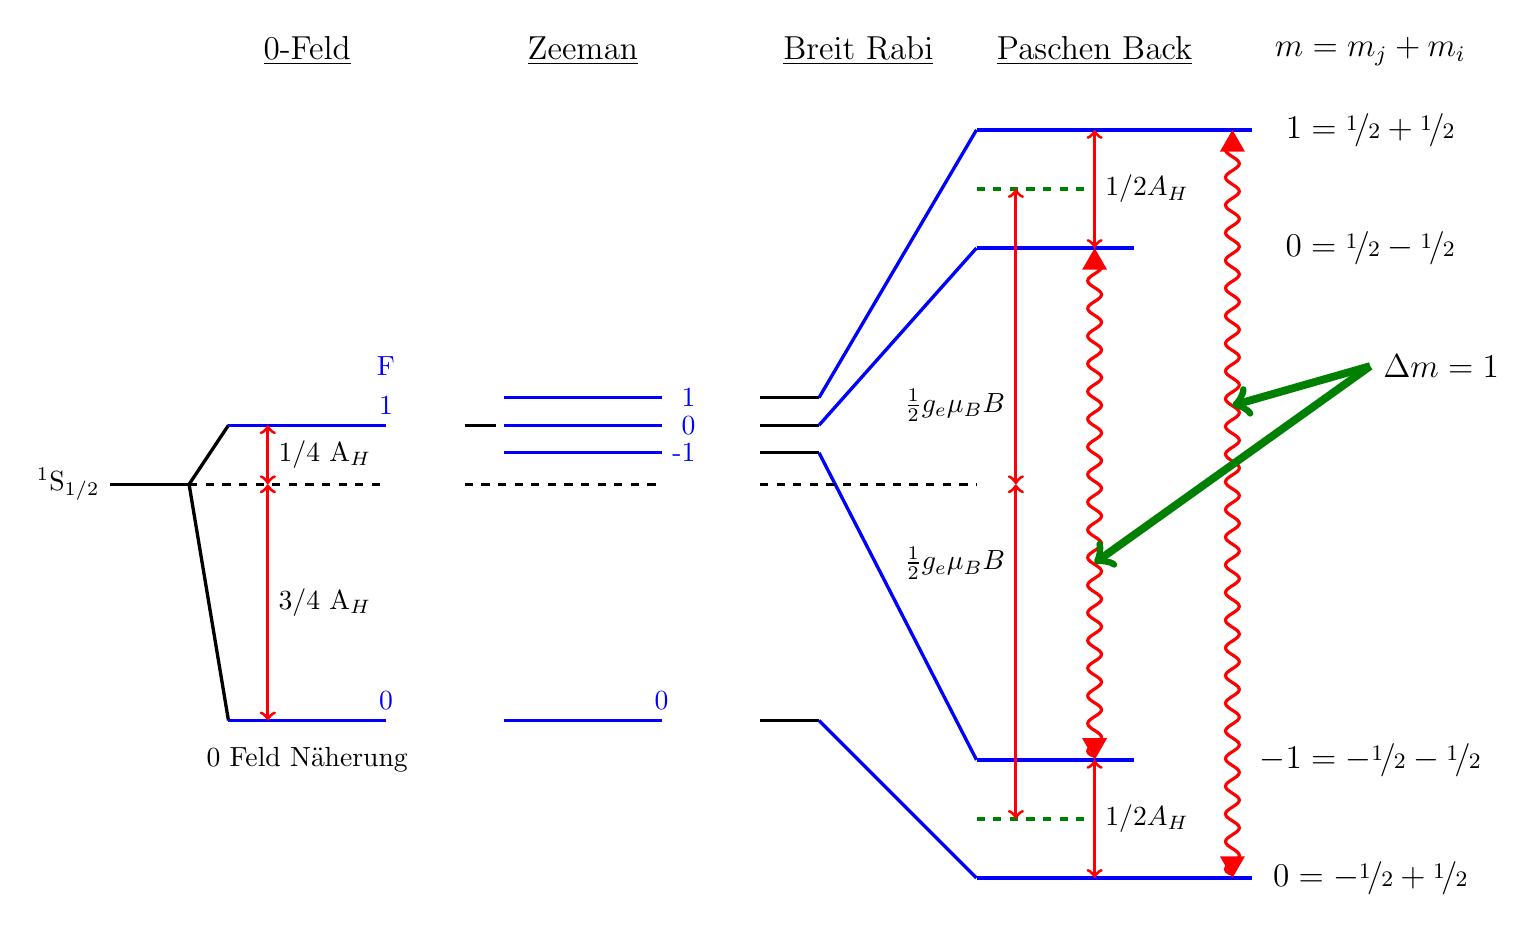
\begin{tikzpicture}[ scale=0.5, level/.style={very thick} ]
    \tikzset{photon/.style={<->,decorate, decoration={snake}, draw=red,
      line width=0.4mm,>=triangle 60}}
    \tikzset{rotdis/.style={<->,decorate, draw=red,line width=0.4mm}}
    % Draw the energy levels.
    %  0 Field
    \draw[level] (3cm, 6cm) -- (5cm, 6cm)node at (3,6)[left]{$^{1}$S$_{1/2}$};
    \draw[level] ( 5cm, 6cm) -- ( 6cm, 7.5cm);
    \draw[level] ( 5cm, 6cm) -- ( 6cm, 0cm);
    \draw[level,blue] ( 6cm, 7.5cm) -- ( 10cm, 7.5cm)node[above]{1};
    \draw[level,blue] ( 6cm, 0cm) -- ( 10cm, 0cm)node[above]{0};
    \draw[-,very thick, dashed](5cm,6cm)--(10cm,6cm);
    \draw[rotdis] (7cm,7.5cm) -- (7cm,6cm)node[right,midway]{$1/4$ A$_{H}$};
    \draw[rotdis] (7cm,6cm) -- (7cm,0cm)node[right,midway]{$3/4$ A$_{H}$};
    \draw[blue] (10.cm,9cm)node{F};
    \draw[](8cm,-1cm)node{0 Feld N\"aherung};
    \draw[](8cm,17cm)node[font=\large]{\underline{0-Feld}};
   %  weak field Field
    \draw[level,blue] ( 13cm, 7.5cm) -- ( 17cm, 7.5cm)node[right]{\ 0};
    \draw[level,blue] ( 13cm, 8.2cm) -- ( 17cm, 8.2cm)node[right]{\ 1};
    \draw[level,blue] ( 13cm, 6.8cm) -- ( 17cm, 6.8cm)node[right]{-1};
    \draw[level,blue] ( 13cm, 0cm) -- ( 17cm, 0cm)node[above]{0};
    \draw[level] ( 12cm, 7.5cm) -- ( 12.8cm, 7.5cm);
    \draw[-,very thick, dashed] ( 12cm, 6cm) -- ( 17cm, 6cm);
    \draw[](15cm,17cm)node[font=\large]{\underline{Zeeman}};
   % Breit Rabi
     \draw[level] ( 19.5cm, 6.8cm) -- ( 21cm, 6.8cm); 
     \draw[level] ( 19.5cm, 7.5cm) -- ( 21cm, 7.5cm); 
     \draw[level] ( 19.5cm, 8.2cm) -- ( 21cm, 8.2cm); 
     \draw[level] ( 19.5cm, 0cm) -- ( 21cm, 0cm); 
     \draw[level,blue]  ( 21cm, 6.8cm) -- (25cm,-1cm); 
     \draw[level,blue]  ( 21cm, 7.5cm) -- (25cm,12cm);  
     \draw[level,blue]  ( 21cm, 8.2cm) -- (25cm,15cm);  
     \draw[level,blue] ( 21cm, 0cm)  --(25cm,-4cm);  
     \draw[-,very thick, dashed] ( 19.5cm, 6cm) -- ( 25cm, 6cm);
     \draw[](22cm,17cm)node[font=\large]{\underline{Breit Rabi}};
    % Paschen Back
    \draw[level,blue] ( 25cm, -1cm) -- ( 29cm,-1cm); 
     \draw[level,blue] ( 25cm, 12cm) -- ( 29cm, 12cm); 
     \draw[level,blue] ( 25cm, 15cm) -- ( 32cm, 15cm); 
     \draw[level,blue] ( 25cm, -4cm) -- ( 32cm, -4cm); 
     \draw[photon] ( 31.5cm, -4cm) -- ( 31.5cm, 15cm); 
     \draw[photon] ( 28.cm, -1cm) -- ( 28.cm, 12cm); 
     \draw[level,green!50!black,dashed] ( 25cm, 13.5cm) -- ( 28cm, 13.5cm); 
     \draw[level,green!50!black,dashed] ( 25cm, -2.5cm) -- ( 28cm, -2.5cm);
     \draw[rotdis] (26cm,-2.5cm) -- (26cm,6cm)node at (26cm,4cm)[left]
      {$\frac{1}{2}g_{e}\mu_{B}B$};
    \draw[rotdis] (26cm,6cm) -- (26cm,13.5cm)node at (26cm,8cm)[left]
      {$\frac{1}{2}g_{e}\mu_{B}B$};
    \draw[rotdis] (28cm,-4cm) -- (28cm,-1cm)node[right,midway]{$1/2 A_{H}$};
    \draw[rotdis] (28cm,12cm) -- (28cm,15cm)node[right,midway]{$1/2 A_{H}$};
    \draw[](35cm,-4cm)node[font=\large]{ $0=-\nicefrac{1}{2}+\nicefrac{1}{2}$};
    \draw[](35cm,-1cm)node[font=\large]{$-1=-\nicefrac{1}{2}-\nicefrac{1}{2}$};
    \draw[](35cm,12cm)node[font=\large]{ $0=\nicefrac{1}{2}-\nicefrac{1}{2}$};
    \draw[](35cm,15cm)node[font=\large]{ $1=\nicefrac{1}{2}+\nicefrac{1}{2}$};
    \draw[](35cm,17cm)node[font=\large]{$m=m_{j}+m_{i}$};
    \draw[](28cm,17cm)node[font=\large]{\underline{Paschen Back}};
     \draw[<-, draw=green!50!black,line width=1mm](31.5cm,8cm)--(35cm,9cm)
      node[right,font=\large]{$\Delta m=1$};
    \draw[<-, draw=green!50!black,line width=1mm](28.cm,4cm)--(35cm,9cm);
  \end{tikzpicture}
\end{document}